\chapter{Contrastive Learning for Batch Detection}
\label{chapter:contrastive-learning-for-batch-detection}

Addressing the need for enhanced traceability within the seafood supply chain, \Cref{chapter:contrastive-learning-for-batch-detection} introduces a novel approach to batch detection using REIMS data. This chapter presents “SpectroSim,” a self-supervised contrastive learning framework specifically designed for identifying whether fish samples originate from the same processing batch. The chapter will detail the motivation for this approach, the SpectroSim architecture (which adapts SimCLR with a Transformer encoder and a custom projection head for mass spectrometry). Experimental results will demonstrate its performance, computational cost, and compare it against both traditional binary classification methods and other state-of-the-art contrastive learning frameworks. Finally, to ensure the model's decisions are interpretable, Gradient-weighted Class Activation Mapping (Grad-CAM) is employed to visualize the key spectral features the model uses to determine batch similarity.

\section{Chapter Overview}
\label{sec:introduction}

Traditional approaches to supply chain traceability in the seafood industry, such as physical tagging, are often complex and costly, creating a significant barrier to widespread adoption \citep{Mai2010,Thompson2005}. While the field is rapidly advancing toward digital solutions like blockchain, `Digital Food Product Passports', and mobile data-entry platforms \citep{turkson2025digital, jiang2025traceability, Untal2025, Gastaldi2025}, these systems are still fundamentally vulnerable to deliberate fraud at the point of data entry \citep{Helyar2014}. A digital record is only as trustworthy as the initial data it is given. This creates a critical need for an intrinsic, chemical-based verification method that can validate a sample's identity against its digital record, a gap that has not been explored for REIMS batch detection. Existing analytical methods for REIMS data are not designed for the nuanced pairwise comparisons required to determine if two samples share a common origin, necessitating the formalization of a new analytical task.

This chapter addresses this gap by formalizing and solving the problem of batch detection in marine biomass as a self-supervised, pairwise comparison task. The emerging paradigm of contrastive learning provides a powerful framework for this challenge, as it is designed to learn a representation space where similar items are grouped together \citep{Bromley1993}. However, applying standard contrastive learning frameworks like SimCLR presents its own difficulties, including a reliance on large batch sizes, which are ill-suited to the limited and high-dimensional nature of REIMS data \citep{Chen2020a,Kinakh2021}. Furthermore, the model must be robust enough to learn subtle, batch-specific chemical signatures, optionally doing so without explicit labels.

This chapter aims to resolve these issues by proposing a novel, self-supervised contrastive learning framework called ``SpectroSim", which is specifically designed for REIMS mass spectra. The solution adapts the SimCLR framework \citep{Chen2020a} by replacing the standard image-based backbone with a Transformer-based encoder \citep{Vaswani2017}, which is adept at capturing the complex, sequential relationships in the spectral data. To overcome the limitations of small datasets, SpectroSim leverages data augmentation to create positive pairs and negative pairs, with a natural imbalance that favors negative sample mining. This is achieved through a custom projection head, data augmentation, and NT-Xent loss function tailored to the unique characteristics of mass spectrometry.

This contribution innovates existing work by being the first to apply any form of machine learning to the problem of batch detection for REIMS biomass analysis. By successfully developing SpectroSim, this chapter establishes that a self-supervised approach can achieve high accuracy (70.8\%) without using any class labels during training, far surpassing traditional binary classification methods. This work provides a new and powerful capability for the seafood industry: a practical, cost-effective, and accurate method for analytical verification. This method complements emerging digital traceability systems \citep{turkson2025digital, dahariya2025enhancing} by providing an intrinsic, scientific tool to validate that a sample's chemical fingerprint matches its claimed batch, thereby enhancing the integrity of data in the modern supply chain \citep{Piroutkova2025}.

\subsection{Contributions}

The main contributions of the chapter are:

\begin{enumerate}
    \item This chapter formalizes the novel problem of analytical batch detection for REIMS data and proposes ``SpectroSim," a new self-supervised contrastive learning framework to solve it. This contribution addresses the critical industry need for a rapid and intrinsic verification method to complement modern digital traceability systems. As far as the authors are aware, this is the first formalization of this task and the first application of any machine learning framework to solve it using REIMS biomass data.
    
    \item This chapter contributes a novel architectural adaptation of the SimCLR framework, successfully integrating a Transformer-based encoder for 1D spectral data. By replacing the standard CNN backbone with a Transformer and a custom projection head, ``SpectroSim" is specifically designed to capture the complex, sequential, and long-range dependencies in mass spectra. This technical contribution overcomes a key limitation of standard contrastive learning, which is ill-suited for high-dimensional, non-image data.
    
    \item This chapter provides the first systematic comparison of learning paradigms for this pairwise comparison task, demonstrating the superiority of self-supervised contrastive learning. The analysis proves that the ``SpectroSim" framework, trained without labels, achieves a high accuracy (70.8\%) and significantly outperforms all benchmarked supervised binary classification methods (which failed to surpass 60\% accuracy), establishing a new state-of-the-art approach for this problem.
    
    \item This chapter demonstrates that contrastive learning can be highly effective on small, high-dimensional datasets, overcoming a primary limitation of standard implementations. ``SpectroSim" achieves its high performance with a batch size of only 16, in contrast to the large batches (e.g., 2048+) typically required by SimCLR. This finding is a significant contribution, as it makes contrastive learning a viable strategy for specialized, limited-sample domains like mass spectrometry analysis.
\end{enumerate}

\section{The Approach}
\label{sec:method}

This section presents SpectroSim, our proposed method for self-supervised batch detection of marine biomass using REIMS data. The task is to determine whether pairs of fish samples originated from the same batch, formulated as a contrastive learning problem that can distinguish similar (same-batch) from dissimilar (different-batch) pairs without relying on labels.

\subsection{Approach Overview}
\label{sec:overall-framework}

% TODO [ ] Bing - Need to add output.

\begin{figure}
    \centering
    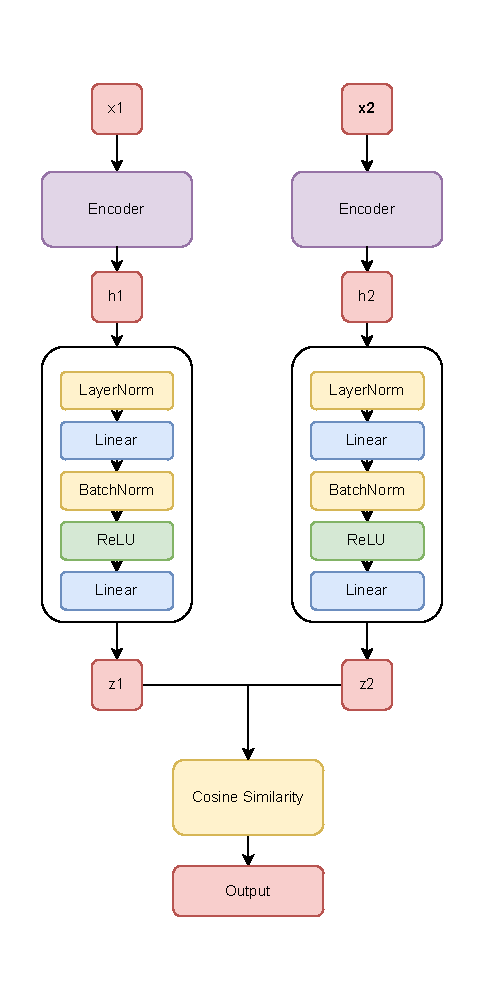
\includegraphics[width=0.5\linewidth]{assets/simclr-architecture.pdf}
    \caption{SpectroSim Architecture: Paired samples $x_1$ and $x_2$
     (REIMS spectra) are processed by identical Transformer encoders $h_1 = f(x_1), h_2 = f(x_2)$
     to produce embeddings
    , followed by a custom projection head $z_1 = g(h_1), z_2 = g(h_2)$
     yielding $z_1$ and $z_2$
    , compared via NT-Xent loss.}
    \label{fig:spectrosim-architecture}
\end{figure}

\Cref{fig:spectrosim-architecture} illustrates SpectroSim’s architecture. It processes pairs of REIMS spectral samples $x_1$ and $x_2$ through identical encoders $h_1 = f(x_1)$, $h_2 = f(x_2)$, where $f$ is the encoder, producing embeddings $h_1$ and $h_2$. A custom projection head $z_1 = g(h_1)$, $z_2 = g(h_2)$, where $g$ is the projection head, maps these to $z_1$ and $z_2$, whose similarity is evaluated using NT-Xent loss. This design extends SimCLR by adapting it for 1D spectral data, addressing SimCLR’s limitations (high computational demands, augmentation dependency, and poor small-dataset performance) through a Transformer encoder and a tailored projection head. These modifications enable efficient learning of batch-specific representations from sequential spectrometry data. A good “semantic” representation for batch detection is illustrated in \Cref{fig:good-semantic-representation}.

\begin{figure}
    \centering
    \includegraphics[width=\linewidth]{assets/representation.png}
    \caption{This figure illustrates a good ``semantic representation". Imagine that the different colors of fish represent fish from different batches in a batch detection task. We feed mass spectrometry samples of these fish into a deep neural network, and it generates embeddings where fish from the same batch are closer together, and fish from dissimilar batches are further apart. In theory, this should make it easy to draw classification boundaries between batches within the embedding space generated by the neural network. Contrastive learning approaches, with their projection head, generate these semantic embeddings, where the distance between samples corresponds to similar and dissimilar batches.}
    \label{fig:good-semantic-representation}
\end{figure}

\subsection{Data Augmentation}

In the SpectroSim framework, the self-supervised learning process relies on creating positive and negative pairs from the input data. A positive pair is formed by creating two different augmented ``views" of the same input sample. For one-dimensional REIMS spectra, augmentations can include adding a small amount of Gaussian noise or applying minor shifts to the $m/z$ axis. These augmentations create a pair of samples that are synthetically different but share the same underlying chemical identity. The model is trained to recognize these augmented views as being similar.

Conversely, a negative pair consists of two samples from different original instances in the batch. For any given sample, all other samples in the training batch are considered negative examples. The model's objective is to learn an embedding space where the representations of positive pairs are pulled closer together, while the representations of negative pairs are pushed further apart. This process forces the model to learn the essential, invariant features that define a sample's batch origin, while ignoring the noise introduced by the augmentation process.

In our contrastive learning framework, we apply a series of data augmentations to the input spectra to generate
different ``views" of the same sample. These augmentations are crucial for learning robust and invariant
representations. 

Figure~\ref{fig:data-augmentations} shows the various data augmentations we apply to a spectra with this unsupervised contrastive learning framework.

\begin{figure}
    \centering
    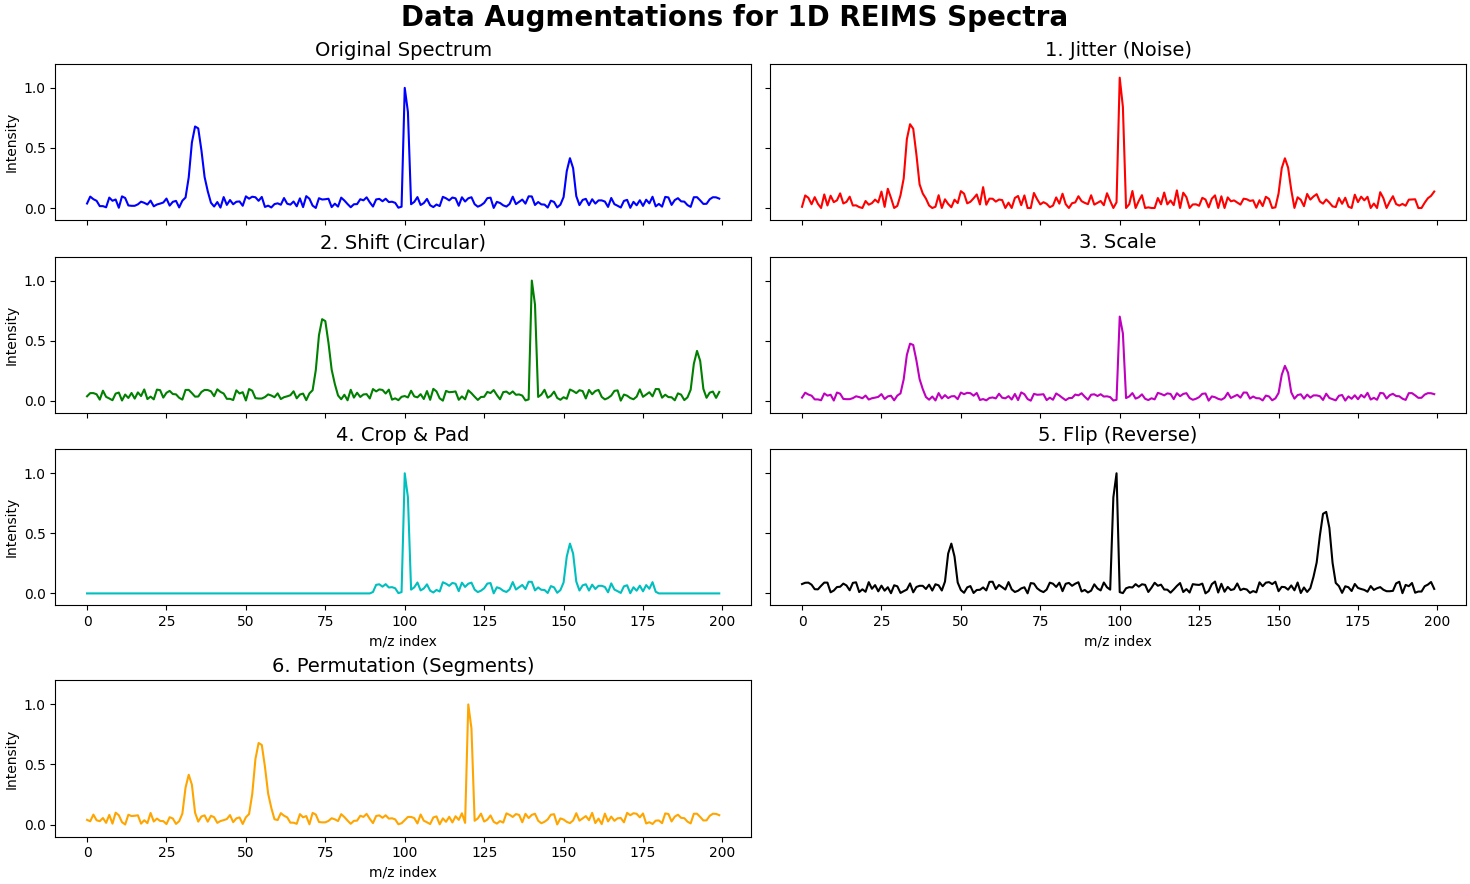
\includegraphics[width=\linewidth]{assets/augmentations.png}
    \caption{Visualization of the six data augmentation techniques described in Section 6.2.2. The \textbf{Original Spectrum} (top left) is shown alongside its six transformed 'views': \textbf{(1) Jitter}, \textbf{(2) Shift}, \textbf{(3) Scale}, \textbf{(4) Crop \& Pad}, \textbf{(5) Flip}, and \textbf{(6) Permutation}. These augmentations are used to create the positive pairs for self-supervised contrastive learning.}
\label{fig:data-augmentations}
\end{figure}


Let an input spectrum be represented by a vector $x \in \mathbb{R}^L$, where $L$ is the number of
features (m/z values). The following transformations are applied to generate an augmented view $x'$:

\subsubsection{Jitter (Noise)}

A random Gaussian noise is added to the spectrum to improve robustness to sensor noise and minor spectral variations.

$x' = x + \epsilon$


\noindent where $\epsilon \sim \mathcal{N}(0, \sigma^2 I)$, and $\sigma$ is the noise level.

\subsubsection{Shift}

The spectrum is circularly shifted along the $m/z$ axis by a random amount. This simulates slight misalignments in the
spectral acquisition.

$x'i = x{(i-s) \pmod L}$


\noindent where $s$ is a random integer shift, and $i$ is the feature index.

\subsubsection{Scale}

The intensity of the entire spectrum is multiplied by a random scalar. This helps the model become invariant to
variations in sample concentration or instrument sensitivity.

$x' = \alpha \cdot x$


\noindent Where $\alpha$ is a random scaling factor drawn from a uniform distribution, typically centered around 1.

\subsubsection{Crop and Pad}

A random contiguous sub-section of the spectrum is selected and then padded with zeros to its original length. This
encourages the model to learn from partial spectral information.


$x'_i = \begin{cases} x_i & \text{if } i \in [start, end) \\ 0 & \text{otherwise} \end{cases}$

\noindent Where $[start, end)$ is a randomly selected interval of the spectral features.

\subsubsection{Flip}


The spectrum is horizontally flipped (reversed) along the $m/z$ axis. This forces the model to learn features that are
not dependent on their position in the spectrum.

$x'i = x{L-1-i}$

\noindent for $i = 0, 1, \dots, L-1$.


\subsubsection{Permutation}

The features of the spectrum are randomly shuffled. This is a strong augmentation that destroys the sequential nature
of the data, forcing the model to learn features based on their values rather than their positions.

$x' = P(x)$

\noindent Where $P$ is a random permutation operator.

\subsection{Encoder}
\label{sec:encoder}

The encoder $h_1 = f(x_1), h_2 = f(x_2)$ is a Transformer, chosen over SimCLR’s ResNet \citep{He2016} because it captures long-range dependencies in 1D spectral sequences—crucial for distinguishing subtle batch-specific chemical signatures—unlike ResNet’s focus on 2D spatial patterns. This choice reduces preprocessing needs and suits the small, high-dimensional dataset, leveraging the Transformer’s attention mechanism for robust feature extraction.

\begin{figure}[t]
    \centering
    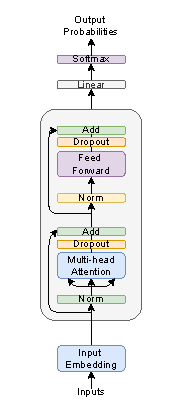
\includegraphics[width=0.3\linewidth]{assets/transformer-architecture.pdf}
    \caption{In the proposed SpectroSim model, we replace the existing ResNet backbone with a Transformer backbone. The choice of transformer is motivated by previous success in REIMS-based marine biomass analysis tasks demonstrated in Chapters 4 and 5. For the sake of academic rigor, we include the original SimCLR with ResNet backbone in our experiments for comparison, and find that the Transformer backbone significantly outperforms the original SimCLR model.}
    \label{fig:enter-label}
\end{figure}

\subsection{Projection Head}
\label{sec:projection} 

In the SpectroSim model, the projection head $z_1 = g(h_1), z_2 = g(h_2)$ shown in \Cref{fig:spectrosim-architecture}, is a custom neural network that operates after the main Transformer encoder, refining its output before the final contrastive loss calculation. Unlike the standard feedforward Multi-Layer Perceptron (MLP) used in the original SimCLR framework, this projection head is specifically designed for spectrometry data. Its primary function is to map the high-dimensional feature representations generated by the encoder into a lower-dimensional space where the NT-Xent loss is applied, a process tailored to reduce information loss by preserving the distributions of spectral peaks. This specialized design ensures the final embeddings are better aligned with the underlying physics of mass spectrometry, creating a more meaningful representation space for comparing samples.

\subsection{Loss Function}

The NT-Xent loss, defined as

\[
\ell_{i,j} = -\log \frac{\exp(\text{sim}(\mathbf{z}_i, \mathbf{z}_j) / \tau)}
{\sum_{k=1}^{2N} \mathbb{1}_{[k \neq i]} \exp(\text{sim}(\mathbf{z}_i, \mathbf{z}_k) / \tau)}
\]

The NT-Xent (Normalized Temperature-scaled Cross-Entropy) loss function is the engine of contrastive learning methods like SimCLR. Its primary goal is to learn an embedding space where similar samples are grouped while dissimilar ones are pushed apart. For a given sample in a batch (the ``anchor," $\mathbf{z}_i$), the loss focuses on maximizing its similarity with its corresponding augmented view (the ``positive," $\mathbf{z}_j$). This is achieved by maximizing the numerator of the fraction. Simultaneously, it minimizes the anchor's similarity to all other samples in the batch (the ``negatives," $\mathbf{z}_k$). The \textbf{temperature parameter} $\tau$ is a crucial hyperparameter that scales the similarity scores; a smaller $\tau$ makes the loss more sensitive to difficult negative examples, forcing the model to learn more discriminative features.

This loss function expertly balances \textbf{intra-class} and \textbf{inter-class} similarity. In this self-supervised context, ``intra-class" refers to the positive pair of augmented views derived from the same original image, while ``inter-class" refers to pairs made from different original images. The loss function encourages high intra-class similarity by explicitly trying to maximize the similarity score $sim(z_i, z_j)$ in the numerator. This has the effect of pulling the representations of positive pairs closer together in the embedding space. At the same time, it promotes low inter-class similarity by including all other samples in the denominator's sum. To minimize the overall loss, the model must learn to make the similarity scores for all negative pairs as low as possible, effectively pushing their representations far apart from the anchor. This dual action creates well-separated clusters for different semantic classes without ever seeing explicit labels.

The symbol $\mathbb{1}_{[k \neq i]}$ is an \textbf{indicator function}, which acts as a simple conditional switch. It evaluates to $1$ if the condition inside the brackets is true (i.e., if $k$ is not equal to $i$) and $0$ if the condition is false. In the denominator, the summation runs over all $2N$ samples in the batch. The purpose of the indicator function is to exclude the anchor sample $\mathbf{z}_i$ from being compared with itself in the sum. Without this condition, the term $\exp(\text{sim}(\mathbf{z}_i, \mathbf{z}_i) / \tau)$ would be included. Since a sample's similarity with itself is trivially perfect, this large value would dominate the denominator and prevent the model from learning the subtle but important differences between the anchor and the actual negative samples. It ensures the model focuses on contrasting positive pairs against all \textit{other} samples, not itself.

\subsection{Threshold}

During training, the best classification threshold is determined by evaluating the performance of the contrastive model on the training data itself. For each pair of augmented samples in a batch, the model produces two embedding vectors, $h_1$ and $h_2$. The cosine similarity between these vectors is calculated for every pair. The algorithm then iterates through a range of potential threshold values from $0.0$ to $1.0$. For each threshold, it makes a prediction: if the cosine similarity of a pair is above the threshold, the samples are predicted to be from the same class (a positive pair); otherwise, they are considered a negative pair. The balanced accuracy of these predictions is calculated against the true pair labels. The threshold that results in the highest balanced accuracy across the training batch is selected as the optimal threshold for that training step and is used for subsequent evaluations.

\section{Experimental Setup}
\label{sec:experimental-setup}

With our methodology clearly defined, we proceed to the experimental setup phase of our study, where we put these diverse machine learning techniques to the test on our REIMS dataset.

\subsection{Benchmark Methods}

To effectively evaluate the proposed method, 18 other binary classification methods are used for comparison on the batch detection for the marine biomass REIMS dataset. These methods include:

\begin{enumerate}
    \item \textbf{Benchmark Technique}: OPLS-DA \citep{Boccard2013}. 
    \item \textbf{Traditional machine learning algorithms}, providing a baseline for comparison. Specifically, Random Forest (RF) \citep{Ho1995}, K-Nearest Neighbors (KNN) \citep{Fix1989}, Decision Trees (DT) \citep{Breiman2017}, Naive Bayes (NB) \citep{Hand2001}, Logistic Regression (LR) \citep{Kleinbaum2002}, Support Vector Machines (SVM) \citep{Cortes1995}, and Linear Discriminant Analysis (LDA) \citep{Balakrishnama1998}.
    \item \textbf{Ensemble method} \citep{Hansen1990}: A combination of the above traditional methods.
    \item \textbf{Contrastive Learning techniques:} Simple Contrastive Learning of Representations (SimCLR) \citep{Chen2020a}.
    \item \textbf{Deep learning models}, (CNNs) \citep{LeCun1989a,LeCun1989b,LeCun1989c,LeCun1998}; Recurrent Convolutional Neural Networks (ResNet) \citep{He2016}; Long-short Term Memory (LSTMs) \citep{Hochreiter1997}; Variational Autoencoders (VAEs) \citep{Kingma2013}; Mamba \citep{Gu2023}; and Kolmogorov-Arnold Networks (KANs) \citep{Liu2024}.
\end{enumerate}

The number of epochs for the deep learning methods is set to 100, the same as the proposed method, to facilitate equitable comparisons. Other hyperparameters are shared across methods where applicable, for the same reason.

\subsection{Benchmark Technique}

To contextualize the performance of our proposed models, we selected \textbf{Orthogonal Partial Least Squares Discriminant Analysis (OPLS-DA)} as the primary benchmark. OPLS-DA is a well-established and standard technique for analyzing REIMS data in the literature, making it an ideal point of comparison between our novel deep learning methods and a traditional approach.

Beyond the OPLS-DA benchmark, the deep learning architectures were evaluated under two distinct frameworks to isolate the impact of the learning strategy itself. These two approaches are illustrated in \Cref{fig:binary-versus-contrastive}.

\begin{enumerate}
    \item \textbf{Direct Binary Classification:} In the first setup, models were trained for standard binary classification. The input was a difference vector, created by subtracting the feature vector of one sample from another. The classifier's task was to use this vector to predict whether the two original samples belonged to the same batch.
    \item \textbf{Contrastive Learning Framework:} In the second setup, the models served as encoders within a contrastive learning framework. Instead of operating on a pre-computed difference, this method learns to generate a separate, rich embedding for each sample in a pair. The cosine similarity between these embeddings is then used to determine if the samples originate from the same batch.
\end{enumerate}

This dual-framework evaluation allows for a direct assessment of the effectiveness of the contrastive learning paradigm compared to a more traditional classification approach using the exact same underlying model architectures.

\begin{figure}
    \centering
    \includegraphics[width=0.7\linewidth]{assets/binary-versus-contrastive.png}
    \caption{This diagram illustrates the difference between binary classification and contrastive learning. Here, we see binary classification takes a difference vector between the two samples and performs binary classification. Whereas contrastive learning learns an embedded representation for each sample and compares these pair-wise. The output for both methods is identical, a prediction of whether the two samples belong to the same or different batches.}
    \label{fig:binary-versus-contrastive}
\end{figure}

\subsection{Experimental Settings}

To evaluate model performance robustly, we used balanced accuracy as the primary metric and conducted 30 independent runs per experiment, with deep learning methods employing early stopping \citep{Morgan1989} to tune epochs based on validation data. For contrastive learning, we applied NT-Xent loss with a temperature of 0.07 to enhance sensitivity to pair similarities, while binary classification used balanced accuracy for traditional methods and weighted cross-entropy for deep learning methods to address class imbalance.

\[ \text{Balanced Accuracy} = \frac{1}{2} \left( \frac{TP}{TP + FN} + \frac{TN}{TN + FP} \right) \] 

% Optuna \cite{Akiba2019} is an open-source hyperparameter optimization framework designed to automate the process of finding the best set of hyperparameters for a machine learning model. It works using a ``define-by-run" API, where you define the search space for your hyperparameters directly within your Python code. Optuna then conducts a series of trials; in each trial, it suggests a set of hyperparameter values, which are then used to train and evaluate your model. The model's performance metric (like accuracy or loss) is returned to Optuna, which uses this result to intelligently decide the next set of hyperparameters to try, often employing sophisticated Bayesian optimization algorithms like the Tree-structured Parzen Estimator (TPE) to efficiently search for the optimal combination. This process allows it to focus on more promising areas of the search space and even prune unpromising trials early, making it far more efficient than manual tuning or grid search.

\subsection{Parameter Settings}

% TODO [ ] Jesse 

To allow for a fair comparison, model hyperparameters were standardized where possible. The deep learning models, including SpectroSim's Transformer encoder, share a consistent set of parameters derived through experimental tuning. Key settings are detailed in \Cref{tab:spectrosim_params}. The AdamW optimizer was used for its effectiveness in regularization. Techniques like label smoothing, dropout, and early stopping were employed to prevent overfitting and ensure robust generalization.

\begin{table}[h!]
\centering
\caption{SpectroSim Transformer Parameter Settings}
\label{tab:spectrosim_params}
\begin{tabular}{ll}
\toprule
\textbf{Parameter} & \textbf{Value} \\
\midrule
Learning rate & 1E-5 \\
Epochs & 100 \\
Dropout & 0.2 \\
Label smoothing & 0.1 \\
Early stopping patience & 5 \\
Optimiser & AdamW \\
Loss: Contrastive & NT-Xent \\
Loss: Binary & CCE \\
Input dimensions & 2080 \\
Hidden dimensions & 128 \\
Output dimensions & 2 \\
Number of layers & 4 \\
Number of heads & 4 \\
\bottomrule
\end{tabular}
\end{table}

\section{Results and Analysis}

This section presents and interprets the outcomes of applying the described machine learning techniques to the batch detection task using the REIMS dataset.


\subsection{Overall Results}

\begin{table}[H]
    \centering
    \caption{Binary Classification Traditional ML Methods (\%)}
    \label{tab:binary_results_traditional}
    \begin{tabular}{|l|c|c|}
        \hline
        Model & Train Acc. & Test Acc. \\ 
        \hline
        OPLS-DA & 57.08 $\pm$ 1.46 & 53.19 $\pm$ 2.22 \\
        KNN & 100.00 $\pm$ 0.00 & 55.69 $\pm$ 2.74 \\
        DT & 100.00 $\pm$ 0.00 & 51.77 $\pm$ 1.43 \\
        \textbf{LDA} & 89.13 $\pm$ 1.15 & \textbf{56.35 $\pm$ 2.70} \\
        NB & 66.95 $\pm$ 2.54 & 55.01 $\pm$ 3.26 \\
        RF & 99.87 $\pm$ 0.33 & 50.02 $\pm$ 0.14 \\
        SVM & 92.44 $\pm$ 1.05 & 54.19 $\pm$ 2.87 \\
        LR & 91.41 $\pm$ 1.19 & 53.90 $\pm$ 3.12 \\
        Ensemble & 95.05 $\pm$ 0.99 & 54.14 $\pm$ 2.81 \\
        \hline
    \end{tabular}
\end{table}

\begin{table}[H]
    \centering
    \caption{Binary Classification DL Encoders (\%)}
    \label{tab:binary_results_encoders}
    \begin{tabular}{|l|c|c|}
        \hline
        Model & Train Acc. & Test Acc. \\
        \hline
        TRANSFORMER & 97.6 $\pm$ 7.4 & 61.5 $\pm$ 7.1 \\
        \textbf{MOE} & 99.9 $\pm$ 0.5 & \textbf{62.5 $\pm$ 7.4} \\
        ENSEMBLE TRANSFORMER & 99.7 $\pm$ 1.1 & 60.8 $\pm$ 7.4 \\
        CNN & 50.0 $\pm$ 1.4 & 52.3 $\pm$ 5.7 \\
        ResNet & 50.2 $\pm$ 1.3 & 51.2 $\pm$ 2.9 \\
        KAN & 49.8 $\pm$ 1.9 & 50.4 $\pm$ 2.5 \\
        VAE & 50.0 $\pm$ 0.0 & 50.0 $\pm$ 0.0 \\
        MAMBA & 50.0 $\pm$ 1.2 & 51.3 $\pm$ 7.7 \\
        \hline
    \end{tabular}
\end{table}

\begin{table}[H]
    \centering
    \caption{Contrastive Learning DL Encoders (\%)}
    \label{tab:simclr_results_encoders}
    \begin{tabular}{|l|c|c|}
        \hline
        Model & Train Acc. & Test Acc. \\
        \hline
        \textbf{TRANSFORMER} & 77.1 $\pm$ 4.9 & \textbf{70.8 $\pm$ 9.6}\\
        MOE & 77.6 $\pm$ 5.6 & 70.4 $\pm$ 10.4 \\
        ENSEMBLE TRANSFORMER & 77.4 $\pm$ 7 & 67.9 $\pm$ 12.8 \\
        CNN & 56.6 $\pm$ 3.1 & 50.6 $\pm$ 12.4 \\
        ResNet & 55.9 $\pm$ 3.3 & 50.0 $\pm$ 8.5 \\
        KAN & 55.7 $\pm$ 2.4 & 50.0 $\pm$ 0.0 \\
        VAE & 51.1 $\pm$ 2.1 & 50.0 $\pm$ 0.0 \\
        MAMBA & 55.4 $\pm$ 2.8 & 50.6 $\pm$ 4.7 \\
        \hline
    \end{tabular}
\end{table}

The initial analysis focused on establishing a performance baseline using traditional machine learning methods with a difference vector approach, as shown in \Cref{tab:binary_results_traditional}. These models universally overfit the training data and failed to generalize, achieving a balanced accuracy only slightly better than random chance ($\approx$ 50\%). While Linear Discriminant Analysis (LDA) emerged as the top performer in this category and marginally outperformed the OPLS-DA benchmark, its overall performance was still inadequate.

When deep learning encoders were applied directly to the same binary classification task (\Cref{tab:binary_results_encoders}), the results were mixed. Most architectures—including CNN, KAN, VAE, Mamba, and the default ResNet encoder—performed on par with the traditional methods, demonstrating poor generalization. However, a notable exception was observed with models designed to interpret sequential data. The Transformer, Mixture of Experts (MoE), and Ensemble models all surpassed 60\% balanced accuracy, suggesting that their ability to capture the sequential nature of REIMS data offers a distinct advantage over other approaches. Despite this improvement, their performance still indicated significant room for growth.

A substantial performance improvement was achieved by integrating the deep learning encoders within the SimCLR contrastive learning framework (\Cref{tab:simclr_results_encoders}). This shift in learning strategy yielded the best results of the study, with the Transformer (70.8\%) encoders demonstrating a dramatic leap in test accuracy. Their success highlights the power of contrastive learning to develop meaningful data representations for batch detection, a task where these same models previously failed as simple classifiers.

The Ensemble Transformer also performed well (67.9\%), though its results were slightly behind the simple Transformer architecture. This may suggest that for learning general-purpose embeddings in this context, the architectural complexity of the ensemble model provides diminishing returns compared to more streamlined models.

The success of the contrastive approach stems from its fundamentally different learning objective. Instead of training on a simple difference vector, the SimCLR framework uses the NT-Xent loss function to structure a meaningful embedding space. This process compels the model to learn the subtle, underlying chemical signatures that define a batch by pulling representations of similar samples (positive pairs) closer together while pushing dissimilar ones (negative pairs) apart.

The result is a robust representation that is far less prone to overfitting and generalizes effectively to unseen data. The results confirm that combining a powerful learning paradigm like contrastive learning with architectures well-suited for sequential data, such as Transformers, is a highly effective strategy. Nevertheless, the framework is not a panacea; the failure of models like KAN and VAE even within this structure underscores that both a suitable model architecture and an appropriate learning strategy are essential for success on this challenging task.

\subsection{Visualization}

While the performance of SpectroSim is high, understanding its decision-making process is crucial for trust and verification by domain experts. To open this black box, we can employ post-hoc explanation techniques like Gradient-weighted Class Activation Mapping (Grad-CAM). These methods can highlight the specific mass-to-charge ($m/z$) ratios that the model finds most important when determining if two samples belong to the same batch. Similar to Chapter 5, we give the average correct Grad-CAM, this time for positive pairs predicted by SpectroSim in batch detection. \Cref{fig:gradcam-spectrosim} provides a visualization of this Grad-CAM.

\begin{figure}
    \centering
    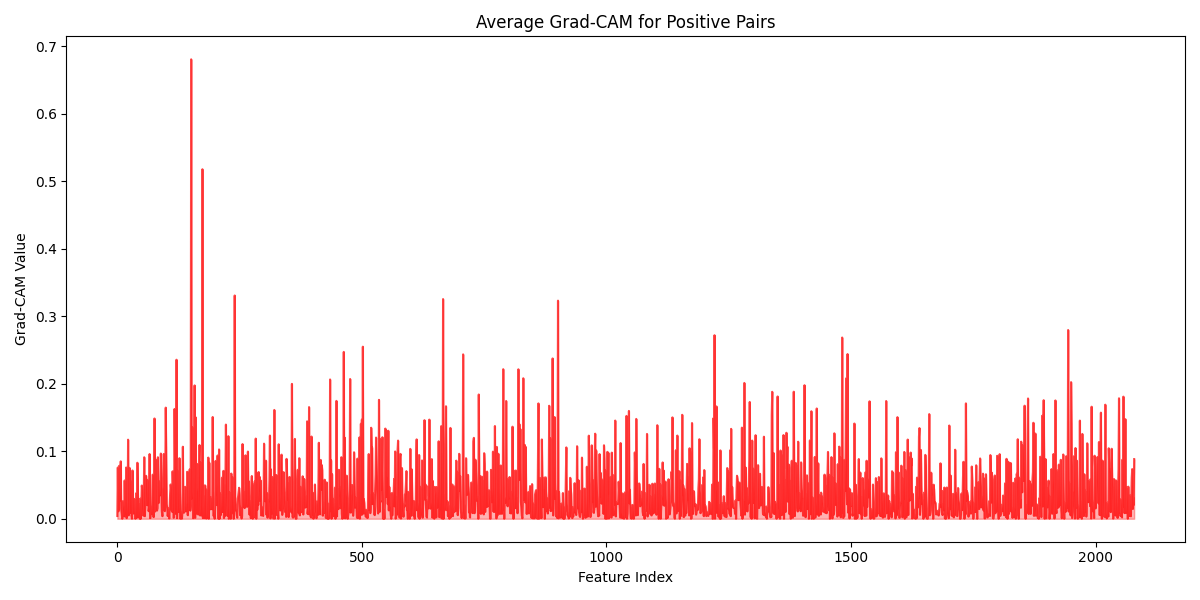
\includegraphics[width=\linewidth]{assets/average_positive_grad_cam.png}
    \caption{Average Grad-CAM for our Transformer-based SpectroSim model. The visualization highlights the most salient m/z features used by the model to compare mass spectra after being trained with SimCLR.}
    \label{fig:gradcam-spectrosim}
\end{figure}

The SpectroSim model analyzes a sample's chemical fingerprint, known as a mass spectrum, by focusing on three key areas. First, it looks at small, common molecular fragments. It then identifies regularly spaced peaks, a pattern created by a family of related molecules (like lipids or polymers) that are built from the same repeating chemical block. Finally, it uses specific, heavy molecular markers to distinguish between very similar samples. This ability to see both broad patterns and unique details shows the model has a sophisticated understanding of the sample's chemistry.

\subsection{Computational Cost}

To evaluate the computational efficiency of various encoder architectures for contrastive learning, we established a standardized benchmark. Each model was tested on a consistent hardware platform using PyTorch to measure key performance indicators: training time, inference time, model size (MB), and the total number of parameters. The evaluation used a single batch from an instance recognition dataset derived from REIMS data, ensuring a direct and fair comparison across architectures.

\begin{table}[t]
\small % Make the font size small to fit the printing area
\centering % Center the table
\caption{Computational Costs for Batch and Instance Detection Models}
\label{tab:comp_cost_combined}
\begin{tabular}{lrrrc} % Simplified tabular environment (Removed `Dataset'): Model, Training Time, Inference Time, Model Size, Parameters
\toprule
\textbf{Model} & \textbf{Training Time (s)} & \textbf{Inference Time (s)} & \textbf{Model Size (MB)} & \textbf{Parameters} \\
\midrule
% Original Data (Batch/Instance Detection Data)
Transformer & 0.203767 & 0.181942 & 421.97 & \num{105491872} \\
MoE & 0.311649 & 0.092523 & 520.36 & \num{130089624} \\
Ensemble & 0.380419 & 0.204004 & 988.88 & \num{247219936} \\
CNN & 0.014521 & 0.087839 & 137.10 & \num{34275328} \\
ResNet & 0.274134 & 0.054243 & 137.10 & \num{34275328} \\
KAN & 0.343616 & 0.044145 & 283.67 & \num{70916316} \\
VAE & 0.225935 & 0.001709 & 10.50 & \num{2626144} \\
Mamba & 1.964942 & 0.430526 & 19.55 & \num{4887808} \\
\bottomrule
\end{tabular}
\end{table}


The results in Table~\Cref{tab:comp_cost_combined} detail the computational costs for each encoder within the SimCLR framework. When considered with the classification accuracies from the previous section, these results highlight the trade-off between performance and computational expense. 
The more complex MoE and Ensemble models are, as expected, more computationally demanding than the standard Transformer. Although the VAE is the most lightweight model with the fastest inference speed, its low classification accuracy suggests the gain in efficiency does not justify the significant loss in performance.

\subsection{Other Contrastive Learning Methods}

To ensure that our SpectroSim method, a self-supervised SimCLR with a Transformer backbone, was up to the task, we compared it against other state-of-the-art contrastive learning methods. We use Stratified k-fold cross-validation to evaluate the accuracy. For this analysis, the contrastive learning methods we compared were:

\begin{itemize}
    \item BYOL \citep{Grill2020} --- This method learns representations by having an online network predict the output of a target network for a different augmented view of the same image. It prevents model collapse by using a momentum-updated target network, which provides stable regression targets without needing explicit negative samples.

    \item Barlow Twins \citep{Zbontar2021} --- This approach learns by making the cross-correlation matrix between the embeddings of two augmented views of an image as close to the identity matrix as possible. This objective encourages the features within the embeddings to be decorrelated, thereby reducing redundancy in the learned representation.

    \item SimSiam \citep{Chen2021} --- A simple Siamese network that maximizes the similarity between two augmentations of an image, using an encoder on one branch and an encoder-predictor pair on the other. It surprisingly avoids collapse without using negative pairs or a momentum encoder by employing a stop-gradient operation, which prevents the outputs from becoming identical.

    \item MoCo \citep{He2020} --- MoCo frames contrastive learning as a dictionary look-up task, where an encoded ``query" from one image view must match its positive ``key" from another view and be distinct from all other negative keys in a dictionary. This dictionary is implemented as a large, dynamic queue, and the key encoder is a momentum-based moving average of the query encoder, which maintains a consistent set of negative samples without needing massive batch sizes.
\end{itemize}


% TODO [ ] Bing - Rerun these experiments.

\begin{table}[t]
    \centering
    \caption{Performance of Contrastive Learning Methods (\%)}
    \label{tab:contrastive_performance_percent}
    \begin{tabular}{|l|c|c|}
        \hline
        Model & Train Acc. & Test Acc. \\
        \hline
        BARLOW TWINS & 54.0 $\pm$ 2.8 & 50.0 $\pm$ 0.0 \\
        BYOL & 56.3 $\pm$ 3.5 & 51.3 $\pm$ 6.3 \\
        MOCO & 54.7 $\pm$ 3.3 & 50.4 $\pm$ 7.7 \\
        \textbf{SIMCLR} & 77.1 $\pm$ 4.9 & \textbf{70.8 $\pm$ 9.6} \\
        SIMSIAM & 54.1 $\pm$ 3.8 & 48.3 $\pm$ 5.1 \\
        \hline
    \end{tabular}
\end{table}

SimCLR is the standout winner by a significant margin, achieving a Mean Test Accuracy of 70.8\%. Its success lies in its direct and aggressive use of negative examples. For each sample, SimCLR treats all other samples in the batch as negatives, creating a strong repulsive force in the embedding space. This process compels the model to learn highly discriminative features that sharply distinguish between different source images, a strategy that proved most effective for this particular task.

The middle-tier methods, BYOL (51.25\%) and MoCo (50.42\%), underperformed because they use strategies to avoid large batches of negative examples. MoCo uses a momentum queue to supply negatives, which may have lacked the diversity of SimCLR's in-batch approach. BYOL avoids negatives entirely, instead training a network to predict its own momentum-updated representations. While these methods are often effective, their performance here suggests that for this dataset, the explicit repulsive force provided by a large set of negatives was crucial for learning separable features.

The worst-performing methods, SimSiam (48.33\%) and Barlow Twins (50.00\%), effectively failed to learn anything meaningful. SimSiam, which uses a simple Siamese network with a stop-gradient, is highly susceptible to ``representational collapse," where it learns a trivial solution by outputting the same features for all inputs. Barlow Twins employs a fundamentally different objective of decorrelating feature dimensions. Its complete failure suggests this complex objective was ill-suited or improperly tuned for the dataset, preventing the model from converging on a useful representation.

\section{Chapter Summary}
\label{sec:conclusions}

\subsection{Conclusions}

This chapter concludes that a self-supervised contrastive learning framework is highly effective for batch detection, achieving promising accuracy and far surpassing traditional binary classification methods. The proposed Transformer-based method, ``SpectroSim," achieved the highest accuracy (70.8\%) when used as an encoder within the SimCLR-based contrastive learning framework.
This success highlights the superiority of using a contrastive learning paradigm over simple binary classification for this task. The findings consistently demonstrate that for every model architecture tested, contrastive learning is more effective than binary classification, and deep learning generally outperforms traditional machine learning. Furthermore, the SimCLR-based approach is shown to outperform other state-of-the-art contrastive learning techniques on this batch detection task. This work establishes the value of deep, sequence-aware models for analyzing high-dimensional REIMS data, as they can leverage natural dataset imbalances for robust representation learning.

\subsection{Future Work}

Future work could explore:

\begin{enumerate}
    \item \textbf{Advanced Model Architectures:} Graph Neural Networks (GNNs) \citep{Wu2020} should be applied to this problem as they can explicitly model the chemical relationships between different mass-to-charge (m/z) peaks, such as isotopic patterns or neutral losses. This approach could capture complex inter-feature dependencies that sequential models only learn implicitly, potentially leading to more robust and chemically-informed classifications.
    
    \item \textbf{Hybrid Models:} This should be explored because different architectures capture distinct patterns; CNNs excel at identifying local features among adjacent peaks, while Transformers model global, long-range dependencies across the entire spectrum. A hybrid model could synergistically combine these strengths to create a more comprehensive feature representation for improved classification accuracy.
    
    \item \textbf{Domain-specific Augmentations:} The integration of domain-specific augmentations, such as spectral peak shifting or noise injection tailored to REIMS chemical profiles, could help create more robust models by artificially expanding the limited training datasets. This would improve generalization by exposing the models to a wider range of plausible spectral variations they might encounter in a real-world setting.
\end{enumerate}

